\chapter{Fundamentals of the \mph analysis}
\label{chapt:mph}
\lettrine{L}{}arge missing transverse momentum (\met) signature can be sign of evidence of new physics, such as the indirect detection of DM.

At LHC we can produce DM particles if they interact with Standard Model particles. A possible candidate to be a constituent of dark matter in universe is given by a weakly interactive mass particle (WIMP), see \Sect{\ref{sec:wimp}}, which interacts with SM particles with a strenght similar to the weak interaction leaving no track on the detector. Missing transverse momentum can only be measured if other particles are produced in the collision, for instance a detectable object such jets or photons, in order to tag the WIMP particle production. 

For the analysis we are using data collected during 2015 and 2016 with the ATLAS detector, corresponding to an integrated luminosity of \SI{36.4}{\ifb}.

%In this chapter after describing the statistical model used in this like in many other analysis at LHC and introducing the software to perform the statistics,, and giving a definition of signal and control regions describing the kinematic cuts used to constrain data I present the result for a background only analysis. I report also a brief evaluation of the raise of systematic uncertainties. It conlcudes with some model-independent upper limit results for a discovery analysis. 
Vediamo come va per scrivere il riassunto del capitolo, su\dots

\section{Statistical model}
In particle physics one often search for phenomena that have been predicted but not observed yet~\cite{Cowan}. Any analysis must be correlated by a quantitative evaluation of the significance of any signal collected. This is usually done by means of a \p or equivalently a Gaussian significance \emph{Z}.

Two kind of hypothesis can be defined. The null hypothesis $H_{0}$, which is the one to be tested against the alternative $H_{1}$. In a discovery analysis, see \Sect{4053}, in which new signal is looked for with no assumption on it, $H_{0}$ plays the role of background only hypothesis and $H_{1}$ is the one who contemplates also signal. When setting limits on a particular model the roles are switched, see \Sect{4054}.

To summarize the outcome of an experiment and quantify the level of agreement between the data and an observed signal one can define a \p:
\begin{definizione}
  The \p of a distribution is the probability under the assumption of $H$ of finding data with equal or greater incompatibility with $H$.
\end{definizione}

An equivalent way to compute this kind of agreement is to turn the \p into Gaussian significance $Z$ by means of the inverse of the cumulative distribution of the standard Gaussian $\Phi^{-1}$ such that:
\begin{equation}
  Z = \Phi^{-1}(1-p)
\end{equation}

Null hypothesis is rejected only if \p is found to be under a common defined threshold usually set at \num{2.87e-7}, corresponding to a significance of $Z=5$.

\subsection{Likelihood based test for the \mph analysis}
The statistic test used in this analysis, such in all physics analysis performed at ATLAS, is based on a profile likelihood approach as pointed out in~\cite{mgiulia}. A likelihood is a funtion of a parameter of interest (POI), here referred to as $\mu$, which could be the visible cross section \sv, see \textbf{later}, or the number of events observed, if rescaled on the integrated luminosity.
The likelihood model takes background and signal yields into account through poissonian distributions, while statistical and systematic uncertainties are nuisance parameters that modify the expectation and which are not known {\itshape a priori} but instead fitted from the data by maximizing the likelihood function.

The full form of the likelihood function used in mono-photon analysis is: 
\begin{equation}
  \label{eqn:likelihood}
  \begin{split}
    \mathfrak{L} \,=\, &  f\left( N \Big\vert \sigma_{\textup{vis}} \cdot L \cdot \prod_s \nu\left(\theta_{s}\right) +\sum _j \beta_{j} B_{j}\cdot \prod_b \nu\left(\theta_{b}\right)\right) \cdot \\
    & \prod_m f\left(N_{m} \Big\vert \sum _j \beta_{j} B_{jm}\right) \cdot \prod _t g\left(\vartheta_{t} \vert \theta_{t}\right) \cdot \prod _k f\left(\xi_{k} \vert \gamma_{k}\right)
  \end{split}
\end{equation}

In equation \Eqn{\ref{eqn:likelihood}}:
\begin{itemize}
\item The first term of $\mathfrak{L}$, as in a counting experiment , is a single poissonian describing the probability of finding N events given $\lambda$ expected\footnote{Remind the Poissonian distribution $P\left(N\vert\lambda\right)=e^{-\lambda}\lambda^N/N!$.}, where $\lambda$ is the term in the second slot of the brackets. It is the sum of signal events $\sigma_{\textup{vis}}L$ (where $L$ is the luminosity) and background events $\sum _j \beta_{j} B_{j}$ in which $B_{j}$ is background yields and $\beta_{j}$ is a scale factor.\footnote{bkg calcolato e fittato nelle CRs e riportato nella SR?? Tipo il k-factor?}.

  Both signal and background yields are multiplied by response function:
  \begin{equation}
    \nu(\theta_{i})  = 1 + \delta \theta_{i}
  \end{equation}
  
where $i=\{s,b\}$, which quantifies the impact of statistical and systematic errors on the signal and background and its value is fitted from the data via the parameter $\delta$. 
  
\item The second term is a poissonian distribution for the $m$-th control region to have $N_{m}$ events over $\sum _j \beta_{j} B_{jm}$ expected in which $\beta_{j}$ could be $1$ or the k factorfor the $j$-th background computed by the fit. Here $B_{jm}$ is multiplied by the respective response function $\nu$.
  
\item The $\prod _t g\left(\vartheta_{t} \vert \theta_{t}\right)$ term constrain the systematic uncertainties with a gaussian term like:
  \begin{equation}
    g(\vartheta_{t} \vert \theta_{t}) = \frac{1}{\sqrt{2\pi}}e^{\frac{(\vartheta_{t}-\theta_{t})^2}{2} } 
  \end{equation}
  
  where $\vartheta$ is the uncertainty on the best estimate of the parameter $\theta$. It is clear that parameter found far away from their best value by the fitting procedure have a lower weight in the likelihood so that the fit prefers already optimized parameters.
  
\item Finally the fourth term treats the sample error due to the finite sample size\footnote{poco chiaro}
\end{itemize}

\subsection{The profiled likelihood ratio}
To test an hypothesized value of $\mu$ we consider the profile likelihood ratio which is used as the {\itshape key} parameter in the whole analysis.
\begin{equation}
  \lambda(\mu) = \frac {\mathfrak{L}(\mu,\hat{\hat{\theta}})}{\mathfrak{L(\hat{\mu},\hat{\theta})}}
\end{equation}

where the denominator is the maximized likelihood and $\hat{\hat{\theta}}$ in the numerator is the value which maximize the likelihood for a given value of $\mu$. $\lambda(\mu)$ is constrained to vary between 0 and 1 so that it is useful to define the corresponding $\tmu$ statistic as 
\begin{equation}
  t_{\mu} = -2 \log{\lambda(\mu)}
\end{equation}
which can be used to build a statistic to measure the discrepancy between data and the hypothesis where higher value of $t_{\mu}$ correspond to higher disagreement. \p can be evaluated even to quantify the level of disagreement, like is pointed out in \Fig{\ref{pvalue}}, as:
\begin{equation}
 p_{\mu}=\int_{t_{\mu,\textup{obs}}}^\infty f\left(t_\mu \vert \mu\right) dt_\mu
\end{equation}

where $t_{\mu,\textup{obs}}$ is the value of $t_\mu$ observed from data and $f\left(t_\mu \vert \mu\right)$ is the probability density function of $t_\mu$ under the assumption of the POI value $\mu$. One can often assume that presence of new signal can only increase the mean event rate, which for a counting experiment can be evaluated as $E[n] = \mu s + b$ where $s$ are the signal events and $b$ is the background, so that we can consider parameter $\mu$ as positive.

Note thath $f\left(t_\mu \vert \mu\right)$ is unknown, because we miss the real POI which is crucial to its determination. According to Wilks' theorem, the distribution of $f(t_\mu \vert \mu)$ is known in the case of a large statistics an it follows a one-degree of freedom (in case of one POI) $\chi^2$ distribution, regardless of the values taken by the nuisance parameters . So $f$ is expressed in term of certain asymptotic formul\ae in the limit of large samples. Alternatively one can obtain it by performing several pseudo-experiment, i.e. \emph{toys}, even if they're always time expensive.

\begin{figure}[tp]
\centering
\subfloat[][]
{\includegraphics[width=.4\textwidth]{monophoton/pvaluea}}
\subfloat[][]
{\includegraphics[width=.416\textwidth]{monophoton/pvalueb}}
\caption{(\emph{a}) Relation between \p and $t_{\mu,\textup{obs}}$. (\emph{b}) Relation between the significance $Z$ and \p for a gaussian distribution $\varphi(x)$.}
\label{pvalue}
\end{figure}

\emph{NOTA}: prima di fare l'analisi model independent e dependent. Ricorda di dire qualcosa sull'Asimov e sui toys. Introduci il qmu espandendo questa sezione 

\section{\hf software framework}

\subsection{Overview}
This analysis is based on a statistical software framework called ``\hf''~\cite{baak:histfitter} which has also been extensively used in several searches for supersymmetric particles, exotic and Higgs Boson physics. 
\hf uses Python and C++ code languages to operate. The user interfaces with the software via a Python macro for configuration while C++ is used in hard computation behind the scenes using the software packages HistFactory and RooStats which are based on RooFit and ROOT.

Usually analyses rely on the comparison between prediction of MC processes and data yields and this software tries to ``fit'', or realize a regression, of MC samples on data. 

Its functioning is based on the concept of Signal Regions (SRs), Validation Regions (VRs) and Control Regions (CRs):
\begin{description}
\item[Signal Region] It's a signal-enriched region defined where a particular signal model predicts a significant excess of events over the predicted background. Depending on the analysis one or more SRs can be defined;
\item[Control Region] It's a background-enriched region and free of signal contamination, used to extimate background in the SR. Comparisons between MC and data are performed and results are extrapolated in the SR Various CRs are defined to contain the greatest number of events for a specific process;
\item[Validation Region] It's a region used to validate the extrapolation process from CRs to SRs. It is placed \emph{halfway} those and its choice is a trade-off between maximizing statistical significance and minimizing signal contamination. In this work no VRs are defined, because the procedure is assumed to be already validate in previous analyses.
\end{description}

\hf also builds a parametric model which is a Probability Density Function (PDF) whose parameters are extracted via a fitting procedure. The above mentioned fit on data is based on SRs and CRs which are statistically independent by construction, i.e. no events can compete for more than one region, so that they can modeled by separate PDFs and combined in a simultaneous fit. The \hf analysis strategy holds on the sharing of PDF parameters in all regions enabling the use of information found in a region everywhere.

Through the fit to data, the observed event counts in CRs are used to normalize the background estimates in the SRs. This extrapolation procedure, which will be shown in action in this analysis in \Fig{\ref{fig:regions}}, happens by means of a rescaling of MC prediction in all regions, i.e. computing a \emph{normalization factor} in the fit.


\subsection{Transfer factor technique and normalisation of background}
In CRs the respective dominant background can be controlled by comparing MC samples to data. Initial predictions of background in a certain CR must be scaled to observed data in that region, using a normalization factor ($k_{i}$) which is usually computed by a numerical fit by the HistFitter software framework. Usually this procedure is referred as an extrapolation from CRs to SR.

One can define a Trasfer Factor by a mere ratio between MC prediction in SR and MC prediction in a CRs, both unnormalized (raw), and the estimate of the number of events in the signal region for the $i$-th process could be written in terms of event observed in the CRs as:
\begin{equation}
  \label{eqn:TF}
  N_{\textup{est},i}(\text{SR}) =  N_{\textup{obs},i}({\text{CR}}) \times \left[\frac{\text{MC}_{\textup{raw},i}(\text{SR})}{\text{MC}_{\textup{raw},i}(\text{CR})} \right]
\end{equation}

The proper normalization factor is defined as the ratio between events observed and expected in the CRs and \Eqn{\ref{eqn:TF}} can also be rewritten as:
\begin{equation}
  N_{\textup{est},i}(\text{SR}) = k_{i}\times\text{MC}_{\textup{raw},i}(\text{SR})
\end{equation}

By this factor the PDF of every region is rescaled everywhere in the parameter space. Indeed the analysis strategy performed by HistFitter shares the same parameters in all region so that any information found in a single region can be brought to the others.

The advantage of using this procedure is that that systematic uncertainties common to the numerator and the denominator of the TF, such as the uncertainty on luminosity, on the predicted background processes can be canceled at first order in the extrapolation.

\section{Event selection}
The Signal Region for the \mph analysis has been defined by comparing the background expectation and different signal model choosing kinematic cuts which would maximies the \emph{significance} of the data. In a very intuitive way if we define $N$ as the number of events yields and assuming absence of signal then $E[N]=b$ with a standard deviation of $\sigma = \sqrt{b}$. Therefore we compute the significance as
\begin{equation}
  Z=\frac{N-b}{\sqrt{b}}=\frac{s}{\sqrt{b}}
  \label{eqn:significance}
\end{equation}
where $s$ is the number of signal events. \Eqn{\ref{eqn:significance}} quantifies the excess of events in terms of the background uncertainty.

\subsection{Selection in Signal Region}
Candidate events in SR are preselected requiring the following property:
\begin{description}
\item [Data quality] Data are considered good for physics if belonging to the Good Run List (GRL). They have to be collected in periods in which optimal detector functioning and stable beams were provided;
\item [Trigger acceptance] Events selected must pass the  \verb!HLT_g140_loose! trigger, which {\itshape I think} is a trigger used to detect events with large \met; 
\item [Vertex quality] We take into account events having a primary vertex reconstructed with two associated good-quality tracks with \pt \SI{\ge 400}{\MeV} and \AetaRange{2.5};
\item [Jet cleaning] Jets tagged with {\itshape BadLoose}  in events in which they overlap with photons or leptons with \pt \SI{>20}{\GeV} or not coming from hard scattering are rejected.
\end{description}

After the preselection Candidates in SR are selected with the following kinematic cuts. In order to populate the region with \gmet events, we consider an event to be part of this region if:
\begin{itemize}
\item we compute \met $ \ge \SI{150}{\gev}$;
\item we get one loose photon with \pt $ \ge 150 $ \GeV $\,$ with a pseudorapidity cut in \etaRange{1.52}{2.37} to cut out the calorimeter crack region and \AetaRange{2.37}
\item \met significance is found to be above $8.5$ \GeV$^{-\frac{1}{2}}$
\item the leading photon is isolated, so that we select events characterized by $ \text{TopoEtcone40} \le 2.45$ \GeV$ + 0.022 \, $\pt \GeV. By this we ensure that in a cone with radius \DeltaRdef $ = 40$, centered in the photon track, all the Topo Clusters have less energy deposited than the one defined above.
\item photon track and \met doesn't overlap, requiring $\Delta\phi_{\gamma - \met} \le 0.4$
\item photon pointing along z coordinate wrt the identified primary vertex must no be larger than $250 \, mm$
\item there is at most one {\itshape good} jet. Even if the analysis is called \mph we take into account events even if they contains a jet, if not we could reject too much statistics as it will be clear in validation plots in section {\bfseries which hasn't been written yet}. Moreover we take only jets such that $\deltaphijetgamma \ge 0.4$

\end{itemize}

In the following section I'm going to deal with all the sources of interference that could affect the SR describing the background processes.

\section{Background estimation}
Alongside the eventual signal coming from unknown ph\oe nomena many other SM processes could pass the cuts defined for the SR ending up being tagged in a wrong way as new physics. We call them background signal, i.e. predictable events that lead to the same signature we are looking for when producing DM particles from \pp scattering.

In other words reasons for events of background can be ascribed to:
\begin{itemize}
\item properly reconstructed SM events which have the same final state as the signal we are looking for;
\item badly reconstructed events in which one (or more) particle are mistaken for photons or they are not reconstructed at all.
\end{itemize}

For the \mph analysis the following background processes were considered.
\begin{itemize}
\item \znng where the two neutrinos produce high \met in the detector. This is the dominant, other than the only irreducible, background as one can see from plots.
\item \wg in which all possible leptonic decay mode of \Wboson are gathered. Here $\ell$ can be an electron being missed or reconstructed as a photon, a muon being missed as well, or a $\tau$ lepton which can decay via hadrons and reconstructed as jet or via leptons and being missed in the detector.
\item \zg where, once again, I am considering all possible leptonic decays for the \Zboson where leptons end up in the same records as in the \Wboson case
\item \gj events in which a jet or photon misreconstruction leads to fake \met.
\item All kind of processes where a jet can fake a photon including:
  \begin{itemize}
  \item double neutrino decay of \Zboson combined with a jet,
  \item leptonic decay of \Wboson along with a jet. If an electron is involved it could fake a photon as well, while we are keeping the jet as pure object for passing SR cuts.
  \end{itemize}
\end{itemize}

In order to quantify the amount of background events in SR, several Control Regions (CRs) are defined which are assumed to be free of signal contamination. Each of them is defined reverting one or more constraints for the SR to enrich every region with a given background process so that they are characterized by a pure dominant process among the others. This provides also ortogonality of a region to one another and their statistical independence.

Events in CRs are simulated via Monte Carlo samples whose prediction must be fitted on data, to get a more reliable estimate of background in SR. This procedure will be explained in detail in section {\bfseries to be written}. A special procedure must be carried out for electron and jets faking photons. In this work results in all the regions for these sources have been taken from previous analysis. However this kind of background cannot be quantified like the previous ones because it is due to some detector mistakes in reconstruction.


\subsection{Definition of Control Regions}
\begin{figure}[tp]
  \centering
  {\fontfamily{pag}\selectfont  
  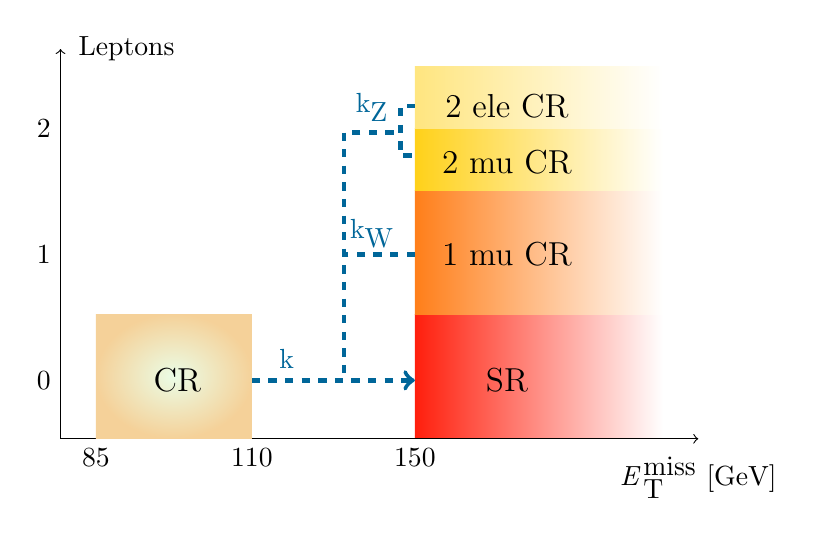
\begin{tikzpicture}[scale=0.9]

      \draw [->](0,0)--(9,0) node[below=3pt]{{\itshape E}$\,_\textup{T}^\textup{miss}$ [GeV]} ;
      \draw [->](0,0)--(0,5.5)node[right=3pt]{Leptons};
      
      \draw node [left] at(0,0.825) {0};
      \draw node [left] at(0,2.6) {1};
      \draw node [left] at(0,3.5+1.75/2) {2};
      \draw node [below] at(0.5,0) {85};
      \draw node [below] at(2.7,0) {110};
      \draw node [below] at(5,0) {150};

      \shade[left color =orange!15!red!95, right color=white] (5,0.015) rectangle +(3.5,1.75-0.015);
      \node[] at (6.3,0.825){\large SR};
      \shade[left color =red!60!yellow!60!orange!90, right color=white] (5,1.75) rectangle +(3.5,1.75);
      \node[] at (6.3,2.6) {\large 1 mu CR};
      \shade[left color =red!20!yellow!90, right color=white] (5,3.5) rectangle +(3.5,1.75/2);
      \node[] at (6.3,3.9) {\large 2 mu CR};
      \shade[left color =orange!40!yellow!50, right color=white] (5,3.5+1.75/2) rectangle +(3.5,1.75/2);
      \node[] at (6.3,4.7) {\large 2 ele CR};
      \shade[outer color=orange!90!green!40,inner color=orange!20!green!10] (0.5,0.01) rectangle +(2.2,1.75);
      \node[align=left] at (1.65,0.825) {\large \gammajet CR};
      
      
      \draw[ultra thick,dashed,->,green!40!blue!100] (2.7,0.825)--(5,0.825);
      \draw node[green!40!blue!100] at (3.2,1.1){k$_{\gammajet}$};
      
      \draw[ultra thick,dashed,green!40!blue!100] (5,4.7)--(4.8,4.7)--(4.8,4)--(5,4);
      \draw[ultra thick,dashed,green!40!blue!100] (4.7,3.5+1.75/2-0.05)--(4,3.5+1.75/2-0.05)--(4,0.87);
      \node[green!40!blue!100] at (4.4,3.5+1.75/2+0.3) { k$_{\textup{Z}}$};
      
      \draw[ultra thick,dashed,green!40!blue!100] (5,2.6) -- (4,2.6);
      \node[green!40!blue!100] at (4.4,2.9) { k$_{\textup{W}}$};
    
   
  \end{tikzpicture}
  }
  \caption{Visual representation of the cuts on \met and number of leptons required for the SR and CRs. The normalization factors k$_\textup{i}$ extracted from CRs and applied to the SR are also shown.}
  \label{fig:regions}
\end{figure}
There are four CRs show in \Fig{\ref{fig:regions}} defined in order to extrapolate information on background in Signal Region. In this section a brief definition and differences in kinematic cuts are descrbed.

\begin{description}
\item [One muon CR] In this region one selected muon is requested, kinematic cuts on \pt and \met are the same of those in SR. Here, however, \met is computed in a different way that is the muon energy is added to this variable, so we can treat it as an invisible particle in order to ensure that \met distribution is similar to the one in SR. This region extracts the normalization $k_W$ for \wg background.
\item [Two muon/electron CR] Similarly to the One muon, here we add to \met both muon/electron contribution to \met. Here two selected muons/electrons are required. we can also add a constrain to the invariant mass of the di-lepton to be greater than \SI{20}{\GeV} and less than \SI{1}{\TeV} to avoid any BSM $Z\gamma$ resonances. Moreover we don't require the cut on \met significance. These regions get $k_Z$ for the dominant background \zg in this region which applies via branching ratio to the \znng process.
\item [Photon jet CR] Here kinematic cuts on \met are lowered. We require \met to be in 85 - 110 \GeV\, range to enrich this region of \gj background because in this energy range, probability to have fake \met from jets is higher. To avoid signal contamination we set $\Delta\phi_{\gamma - \met} \le 3.0$ so that we prevent {\itshape back-to-back} signal events to fall in this region. This region, defined in \RunTwo, constrains the normalization for \gj background to get a $k_{pj}$ normalization factor.
\end{description}

{\itshape A priori} a one electron CR could have been defined as well. Nevertheless the one muon CR has enough statistic to constrain the normalization on \Wboson$\gamma$.  This kind of region would have been more difficult to manage even just because electrons could be reconstructed easily as photons which not happens for muons being detected far away in the detector from photons increasing the number of \gj events contamination. In the analysis carried out in [nota di supporto] one evince that no improvement on $k_W$ error can be seen, instead there is a raise of $k_{pj}$ error due to furhter background contamination.

As mentioned earlier fake photons from electrons and jets enter the fit as given values and it is not constrained by any region. They have been estimated via data driven tecniques in other analysis.

\section{Results for a backgroud only fit}

\section{Systematic uncertainties}


\subsection{Experimental sensitivity, da mettere prima delle analisi}
It is useful to characterize the sensitivity of an experiment by reporting the expected significance that one would obtain for a variety of signal hypotheses. One is not interested in the significance obtained in a single data set while in the expected (median) significance whose estimation is given by replacing the ensamble of simulated data set with a single representative one, the so-called Asimov data set. Otherwise one can simulate several \emph{toys} in order to get as much statistic as he could.

If we're analysing data regardless of any nuisance parameters, one can assume that if there is no signal then $E[n]=b$ with standard deviation $\sigma = \sqrt{b}$. Therefore we compute the significance as
\begin{equation}
  z=\frac{n-b}{\sqrt{b}}=\frac{s}{\sqrt{b}}
\end{equation}

and the probability that $s$ comes from background fluctuations is evaluated via the \p in the following way:
\begin{equation}
  p=\int_Z^\infty \frac{e^{-\frac{z^2}{2}}}{\sqrt{2\pi}}\,dz .
\end{equation}
QUI C'\`E UNA PARTE DA CAPIRE CHE \`E LA FIGURA 2 DEL COWAN.
